\renewcommand{\theequation}{\theenumi}
\begin{enumerate}[label=\thesection.\arabic*.,ref=\thesection.\theenumi]
\numberwithin{equation}{enumi}
\item This is a binomial distribution where success is at getting an odd number.
\item No. of trials $= n = 3$. 
\item Probability of getting an odd number $= p = \frac{3}{6} = \frac{1}{2}$. 
\begin{figure}[!ht]
\centering
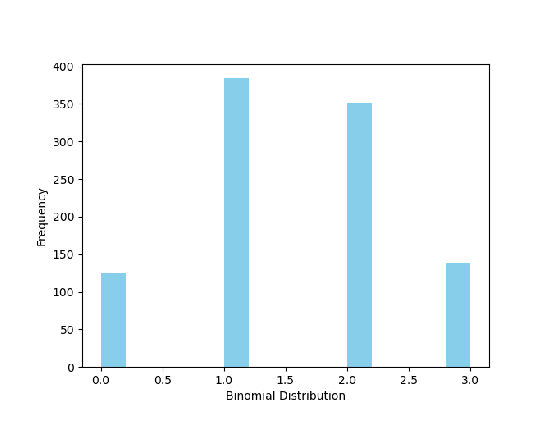
\includegraphics[width= \columnwidth]{./probability/figs/Q40binom.eps}
\caption{Binomial distribution: n=3, p=0.5 (size =1000)}
\end{figure}
\item Then by binomial distribution
\begin{align}
P(r\geq1)&= 1 - P(r=0)\\
&= 1 - \Mycomb{r}p^{r}(1-p)^{n-r}\\
&= 0.875
\end{align}

\item From the graph in fig. , we can find the answer.
\item Download the python code from
\begin{lstlisting}
probability/codes/Q40binom.py
\end{lstlisting}

\end{enumerate}